\documentclass[]{article}
\usepackage{lmodern}
\usepackage{amssymb,amsmath}
\usepackage{ifxetex,ifluatex}
\usepackage{fixltx2e} % provides \textsubscript
\ifnum 0\ifxetex 1\fi\ifluatex 1\fi=0 % if pdftex
  \usepackage[T1]{fontenc}
  \usepackage[utf8]{inputenc}
\else % if luatex or xelatex
  \ifxetex
    \usepackage{mathspec}
  \else
    \usepackage{fontspec}
  \fi
  \defaultfontfeatures{Ligatures=TeX,Scale=MatchLowercase}
\fi
% use upquote if available, for straight quotes in verbatim environments
\IfFileExists{upquote.sty}{\usepackage{upquote}}{}
% use microtype if available
\IfFileExists{microtype.sty}{%
\usepackage{microtype}
\UseMicrotypeSet[protrusion]{basicmath} % disable protrusion for tt fonts
}{}
\usepackage[margin=1in]{geometry}
\usepackage{hyperref}
\hypersetup{unicode=true,
            pdftitle={Analyse du risque de défaillance des joints toriques de la navette Challenger},
            pdfauthor={Arnaud Legrand},
            pdfborder={0 0 0},
            breaklinks=true}
\urlstyle{same}  % don't use monospace font for urls
\usepackage{color}
\usepackage{fancyvrb}
\newcommand{\VerbBar}{|}
\newcommand{\VERB}{\Verb[commandchars=\\\{\}]}
\DefineVerbatimEnvironment{Highlighting}{Verbatim}{commandchars=\\\{\}}
% Add ',fontsize=\small' for more characters per line
\usepackage{framed}
\definecolor{shadecolor}{RGB}{248,248,248}
\newenvironment{Shaded}{\begin{snugshade}}{\end{snugshade}}
\newcommand{\AlertTok}[1]{\textcolor[rgb]{0.94,0.16,0.16}{#1}}
\newcommand{\AnnotationTok}[1]{\textcolor[rgb]{0.56,0.35,0.01}{\textbf{\textit{#1}}}}
\newcommand{\AttributeTok}[1]{\textcolor[rgb]{0.77,0.63,0.00}{#1}}
\newcommand{\BaseNTok}[1]{\textcolor[rgb]{0.00,0.00,0.81}{#1}}
\newcommand{\BuiltInTok}[1]{#1}
\newcommand{\CharTok}[1]{\textcolor[rgb]{0.31,0.60,0.02}{#1}}
\newcommand{\CommentTok}[1]{\textcolor[rgb]{0.56,0.35,0.01}{\textit{#1}}}
\newcommand{\CommentVarTok}[1]{\textcolor[rgb]{0.56,0.35,0.01}{\textbf{\textit{#1}}}}
\newcommand{\ConstantTok}[1]{\textcolor[rgb]{0.00,0.00,0.00}{#1}}
\newcommand{\ControlFlowTok}[1]{\textcolor[rgb]{0.13,0.29,0.53}{\textbf{#1}}}
\newcommand{\DataTypeTok}[1]{\textcolor[rgb]{0.13,0.29,0.53}{#1}}
\newcommand{\DecValTok}[1]{\textcolor[rgb]{0.00,0.00,0.81}{#1}}
\newcommand{\DocumentationTok}[1]{\textcolor[rgb]{0.56,0.35,0.01}{\textbf{\textit{#1}}}}
\newcommand{\ErrorTok}[1]{\textcolor[rgb]{0.64,0.00,0.00}{\textbf{#1}}}
\newcommand{\ExtensionTok}[1]{#1}
\newcommand{\FloatTok}[1]{\textcolor[rgb]{0.00,0.00,0.81}{#1}}
\newcommand{\FunctionTok}[1]{\textcolor[rgb]{0.00,0.00,0.00}{#1}}
\newcommand{\ImportTok}[1]{#1}
\newcommand{\InformationTok}[1]{\textcolor[rgb]{0.56,0.35,0.01}{\textbf{\textit{#1}}}}
\newcommand{\KeywordTok}[1]{\textcolor[rgb]{0.13,0.29,0.53}{\textbf{#1}}}
\newcommand{\NormalTok}[1]{#1}
\newcommand{\OperatorTok}[1]{\textcolor[rgb]{0.81,0.36,0.00}{\textbf{#1}}}
\newcommand{\OtherTok}[1]{\textcolor[rgb]{0.56,0.35,0.01}{#1}}
\newcommand{\PreprocessorTok}[1]{\textcolor[rgb]{0.56,0.35,0.01}{\textit{#1}}}
\newcommand{\RegionMarkerTok}[1]{#1}
\newcommand{\SpecialCharTok}[1]{\textcolor[rgb]{0.00,0.00,0.00}{#1}}
\newcommand{\SpecialStringTok}[1]{\textcolor[rgb]{0.31,0.60,0.02}{#1}}
\newcommand{\StringTok}[1]{\textcolor[rgb]{0.31,0.60,0.02}{#1}}
\newcommand{\VariableTok}[1]{\textcolor[rgb]{0.00,0.00,0.00}{#1}}
\newcommand{\VerbatimStringTok}[1]{\textcolor[rgb]{0.31,0.60,0.02}{#1}}
\newcommand{\WarningTok}[1]{\textcolor[rgb]{0.56,0.35,0.01}{\textbf{\textit{#1}}}}
\usepackage{graphicx,grffile}
\makeatletter
\def\maxwidth{\ifdim\Gin@nat@width>\linewidth\linewidth\else\Gin@nat@width\fi}
\def\maxheight{\ifdim\Gin@nat@height>\textheight\textheight\else\Gin@nat@height\fi}
\makeatother
% Scale images if necessary, so that they will not overflow the page
% margins by default, and it is still possible to overwrite the defaults
% using explicit options in \includegraphics[width, height, ...]{}
\setkeys{Gin}{width=\maxwidth,height=\maxheight,keepaspectratio}
\IfFileExists{parskip.sty}{%
\usepackage{parskip}
}{% else
\setlength{\parindent}{0pt}
\setlength{\parskip}{6pt plus 2pt minus 1pt}
}
\setlength{\emergencystretch}{3em}  % prevent overfull lines
\providecommand{\tightlist}{%
  \setlength{\itemsep}{0pt}\setlength{\parskip}{0pt}}
\setcounter{secnumdepth}{0}
% Redefines (sub)paragraphs to behave more like sections
\ifx\paragraph\undefined\else
\let\oldparagraph\paragraph
\renewcommand{\paragraph}[1]{\oldparagraph{#1}\mbox{}}
\fi
\ifx\subparagraph\undefined\else
\let\oldsubparagraph\subparagraph
\renewcommand{\subparagraph}[1]{\oldsubparagraph{#1}\mbox{}}
\fi

%%% Use protect on footnotes to avoid problems with footnotes in titles
\let\rmarkdownfootnote\footnote%
\def\footnote{\protect\rmarkdownfootnote}

%%% Change title format to be more compact
\usepackage{titling}

% Create subtitle command for use in maketitle
\newcommand{\subtitle}[1]{
  \posttitle{
    \begin{center}\large#1\end{center}
    }
}

\setlength{\droptitle}{-2em}

  \title{Analyse du risque de défaillance des joints toriques de la navette
Challenger}
    \pretitle{\vspace{\droptitle}\centering\huge}
  \posttitle{\par}
    \author{Arnaud Legrand}
    \preauthor{\centering\large\emph}
  \postauthor{\par}
      \predate{\centering\large\emph}
  \postdate{\par}
    \date{28 juin 2018}


\begin{document}
\maketitle

Le 27 Janvier 1986, veille du décollage de la navette /Challenger/, eu
lieu une télé-conférence de trois heures entre les ingénieurs de la
Morton Thiokol (constructeur d'un des moteurs) et de la NASA. La
discussion portait principalement sur les conséquences de la température
prévue au moment du décollage de 31°F (juste en dessous de 0°C) sur le
succès du vol et en particulier sur la performance des joints toriques
utilisés dans les moteurs. En effet, aucun test n'avait été effectué à
cette température.

L'étude qui suit reprend donc une partie des analyses effectuées cette
nuit là et dont l'objectif était d'évaluer l'influence potentielle de la
température et de la pression à laquelle sont soumis les joints toriques
sur leur probabilité de dysfonctionnement. Pour cela, nous disposons des
résultats des expériences réalisées par les ingénieurs de la NASA durant
les 6 années précédant le lancement de la navette Challenger.

\hypertarget{chargement-des-donnees}{%
\section{Chargement des données}\label{chargement-des-donnees}}

Nous commençons donc par charger ces données:

\begin{Shaded}
\begin{Highlighting}[]
\NormalTok{data =}\StringTok{ }\KeywordTok{read.csv}\NormalTok{(}\StringTok{"shuttle.csv"}\NormalTok{,}\DataTypeTok{header=}\NormalTok{T)}
\NormalTok{data}
\end{Highlighting}
\end{Shaded}

\begin{verbatim}
##         Date Count Temperature Pressure Malfunction
## 1    4/12/81     6          66       50           0
## 2   11/12/81     6          70       50           1
## 3    3/22/82     6          69       50           0
## 4   11/11/82     6          68       50           0
## 5    4/04/83     6          67       50           0
## 6    6/18/82     6          72       50           0
## 7    8/30/83     6          73      100           0
## 8   11/28/83     6          70      100           0
## 9    2/03/84     6          57      200           1
## 10   4/06/84     6          63      200           1
## 11   8/30/84     6          70      200           1
## 12  10/05/84     6          78      200           0
## 13  11/08/84     6          67      200           0
## 14   1/24/85     6          53      200           2
## 15   4/12/85     6          67      200           0
## 16   4/29/85     6          75      200           0
## 17   6/17/85     6          70      200           0
## 18 7/2903/85     6          81      200           0
## 19   8/27/85     6          76      200           0
## 20  10/03/85     6          79      200           0
## 21  10/30/85     6          75      200           2
## 22  11/26/85     6          76      200           0
## 23   1/12/86     6          58      200           1
\end{verbatim}

Le jeu de données nous indique la date de l'essai, le nombre de joints
toriques mesurés (il y en a 6 sur le lançeur principal), la température
(en Farenheit) et la pression (en psi), et enfin le nombre de
dysfonctionnements relevés.

\hypertarget{inspection-graphique-des-donnees}{%
\section{Inspection graphique des
données}\label{inspection-graphique-des-donnees}}

Les vols où aucun incident n'est relevé n'apportant aucun information
sur l'influence de la température ou de la pression sur les
dysfonctionnements, nous nous concentrons sur les expériences où au
moins un joint a été défectueux.

\begin{Shaded}
\begin{Highlighting}[]
\NormalTok{data =}\StringTok{ }\NormalTok{data[data}\OperatorTok{$}\NormalTok{Malfunction}\OperatorTok{>}\DecValTok{0}\NormalTok{,]}
\NormalTok{data}
\end{Highlighting}
\end{Shaded}

\begin{verbatim}
##        Date Count Temperature Pressure Malfunction
## 2  11/12/81     6          70       50           1
## 9   2/03/84     6          57      200           1
## 10  4/06/84     6          63      200           1
## 11  8/30/84     6          70      200           1
## 14  1/24/85     6          53      200           2
## 21 10/30/85     6          75      200           2
## 23  1/12/86     6          58      200           1
\end{verbatim}

Très bien, nous avons une variabilité de température importante mais la
pression est quasiment toujours égale à 200, ce qui devrait simplifier
l'analyse.

Comment la fréquence d'échecs varie-t-elle avec la température ?

\begin{Shaded}
\begin{Highlighting}[]
\KeywordTok{plot}\NormalTok{(}\DataTypeTok{data=}\NormalTok{data, Malfunction}\OperatorTok{/}\NormalTok{Count }\OperatorTok{~}\StringTok{ }\NormalTok{Temperature, }\DataTypeTok{ylim=}\KeywordTok{c}\NormalTok{(}\DecValTok{0}\NormalTok{,}\DecValTok{1}\NormalTok{))}
\end{Highlighting}
\end{Shaded}

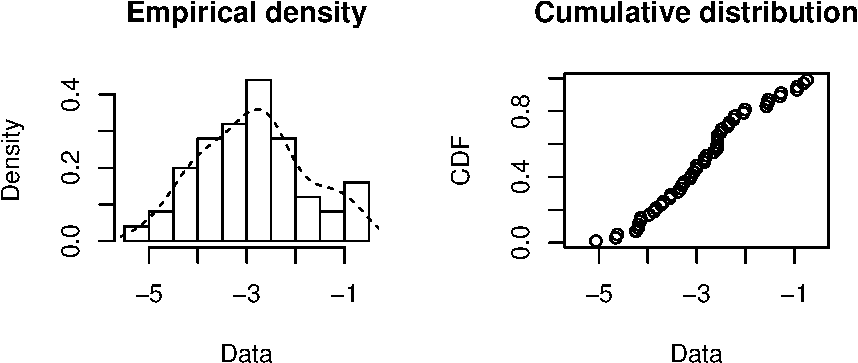
\includegraphics{exo5_files/figure-latex/unnamed-chunk-3-1.pdf}

À première vue, ce n'est pas flagrant mais bon, essayons quand même
d'estimer l'impact de la température \(t\) sur la probabilité de
dysfonctionnements d'un joint.

\hypertarget{estimation-de-linfluence-de-la-temperature}{%
\section{Estimation de l'influence de la
température}\label{estimation-de-linfluence-de-la-temperature}}

Supposons que chacun des 6 joints toriques est endommagé avec la même
probabilité et indépendamment des autres et que cette probabilité ne
dépend que de la température. Si on note \(p(t)\) cette probabilité, le
nombre de joints \(D\) dysfonctionnant lorsque l'on effectue le vol à
température \(t\) suit une loi binomiale de paramètre \(n=6\) et
\(p=p(t)\). Pour relier \(p(t)\) à \(t\), on va donc effectuer une
régression logistique.

\begin{Shaded}
\begin{Highlighting}[]
\NormalTok{logistic_reg =}\StringTok{ }\KeywordTok{glm}\NormalTok{(}\DataTypeTok{data=}\NormalTok{data, Malfunction}\OperatorTok{/}\NormalTok{Count }\OperatorTok{~}\StringTok{ }\NormalTok{Temperature, }\DataTypeTok{weights=}\NormalTok{Count, }
                   \DataTypeTok{family=}\KeywordTok{binomial}\NormalTok{(}\DataTypeTok{link=}\StringTok{'logit'}\NormalTok{))}
\KeywordTok{summary}\NormalTok{(logistic_reg)}
\end{Highlighting}
\end{Shaded}

\begin{verbatim}
## 
## Call:
## glm(formula = Malfunction/Count ~ Temperature, family = binomial(link = "logit"), 
##     data = data, weights = Count)
## 
## Deviance Residuals: 
##       2        9       10       11       14       21       23  
## -0.3015  -0.2836  -0.2919  -0.3015   0.6891   0.6560  -0.2850  
## 
## Coefficients:
##              Estimate Std. Error z value Pr(>|z|)
## (Intercept) -1.389528   3.195752  -0.435    0.664
## Temperature  0.001416   0.049773   0.028    0.977
## 
## (Dispersion parameter for binomial family taken to be 1)
## 
##     Null deviance: 1.3347  on 6  degrees of freedom
## Residual deviance: 1.3339  on 5  degrees of freedom
## AIC: 18.894
## 
## Number of Fisher Scoring iterations: 4
\end{verbatim}

L'estimateur le plus probable du paramètre de température est 0.001416
et l'erreur standard de cet estimateur est de 0.049, autrement dit on ne
peut pas distinguer d'impact particulier et il faut prendre nos
estimations avec des pincettes.

\hypertarget{estimation-de-la-probabilite-de-dysfonctionnant-des-joints-toriques}{%
\section{Estimation de la probabilité de dysfonctionnant des joints
toriques}\label{estimation-de-la-probabilite-de-dysfonctionnant-des-joints-toriques}}

La température prévue le jour du décollage est de 31°F. Essayons
d'estimer la probabilité de dysfonctionnement des joints toriques à
cette température à partir du modèle que nous venons de construire:

\begin{Shaded}
\begin{Highlighting}[]
\CommentTok{# shuttle=shuttle[shuttle$r!=0,] }
\NormalTok{tempv =}\StringTok{ }\KeywordTok{seq}\NormalTok{(}\DataTypeTok{from=}\DecValTok{30}\NormalTok{, }\DataTypeTok{to=}\DecValTok{90}\NormalTok{, }\DataTypeTok{by =} \FloatTok{.5}\NormalTok{)}
\NormalTok{rmv <-}\StringTok{ }\KeywordTok{predict}\NormalTok{(logistic_reg,}\KeywordTok{list}\NormalTok{(}\DataTypeTok{Temperature=}\NormalTok{tempv),}\DataTypeTok{type=}\StringTok{"response"}\NormalTok{)}
\KeywordTok{plot}\NormalTok{(tempv,rmv,}\DataTypeTok{type=}\StringTok{"l"}\NormalTok{,}\DataTypeTok{ylim=}\KeywordTok{c}\NormalTok{(}\DecValTok{0}\NormalTok{,}\DecValTok{1}\NormalTok{))}
\KeywordTok{points}\NormalTok{(}\DataTypeTok{data=}\NormalTok{data, Malfunction}\OperatorTok{/}\NormalTok{Count }\OperatorTok{~}\StringTok{ }\NormalTok{Temperature)}
\end{Highlighting}
\end{Shaded}

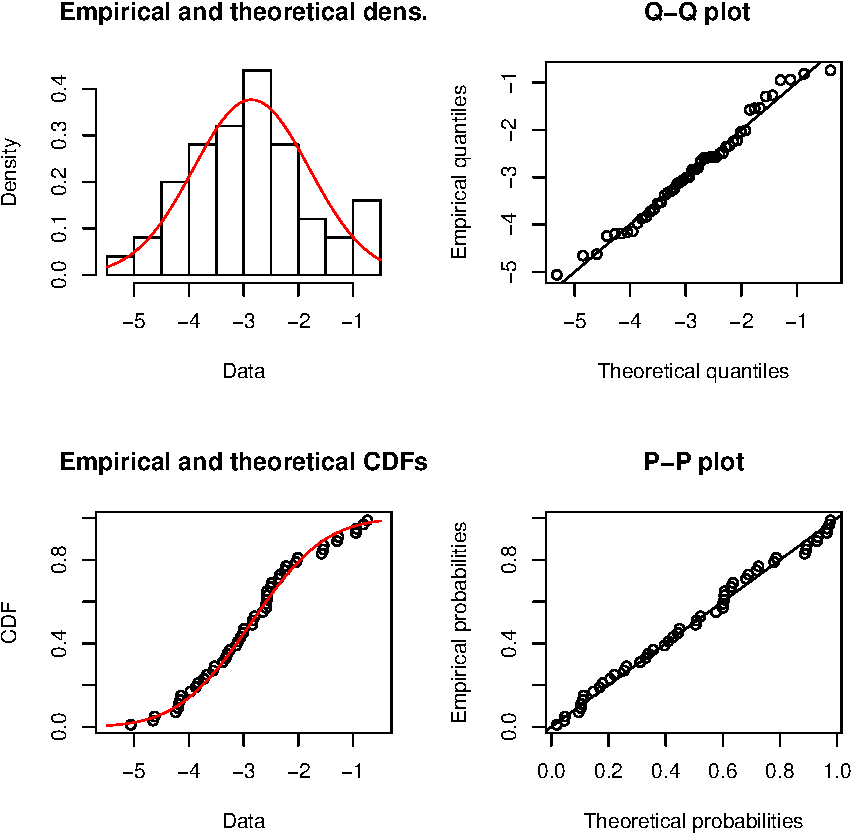
\includegraphics{exo5_files/figure-latex/unnamed-chunk-5-1.pdf}

La probabilité d'échec des joints toriques est donc d'environ 0.2 (comme
dans les essais précédents) et comme on pouvait s'attendre au vu des
données initiales, la température n'a pas d'impact notable. La
probabilité que tous les joints toriques dysfonctionnent est de
\(0.2^6 \approx 6.4\times10^{-5}\). Tout est sous contrôle, le décollage
peut donc avoir lieu demain comme prévu.

Seulement, le lendemain, la navette Challenger explosera et emportera
avec elle ses sept membres d'équipages. L'opinion publique est fortement
touchée et lors de l'enquête qui suivra, la fiabilité des joints
toriques sera directement mise en cause. Au delà des problèmes de
communication interne à la NASA qui sont pour beaucoup dans ce fiasco,
l'analyse précédente comporte (au moins) un petit problème\ldots{}
Saurez-vous le trouver ? Vous êtes libre de modifier cette analyse et de
regarder ce jeu de données sous tous les angles afin d'expliquer ce qui
ne va pas.

\hypertarget{ajout-dun-terme-quadratique}{%
\section{Ajout d'un terme
quadratique}\label{ajout-dun-terme-quadratique}}

Comme on le voit sur le graphique, et comme on peut s'y attendre, la
réponse n'est pas monotone par rapport à la température : on ne s'attend
pas à une simple augmentation du taux de dysfonctionnement avec la
température. La courbe ressmblerait plus à un un ``U'' : le taux de
dysfonctionnement pourrait être plus élevé aux basses températures ainsi
qu'aux fortes températures. La regression logistique simple impose un
terme linéaire, et comme on le voit sur le graphique le modèle prévoit
une augmentation faible et monotone du taux de dysfonctionnement avec la
température, ce qui implique aussi que le taux de dysfonctionnement tend
vers 0 avec les températures décroissantes. En ajoutant un terme
quadratique au modèle de regression, on permet au modèle de s'ajuster à
une réponse non monotone :

\begin{Shaded}
\begin{Highlighting}[]
\NormalTok{logistic_reg_quad =}\StringTok{ }\KeywordTok{glm}\NormalTok{(}\DataTypeTok{data=}\NormalTok{data, Malfunction}\OperatorTok{/}\NormalTok{Count }\OperatorTok{~}\StringTok{ }\KeywordTok{poly}\NormalTok{(Temperature,}\DecValTok{2}\NormalTok{), }\DataTypeTok{weights=}\NormalTok{Count, }
                   \DataTypeTok{family=}\KeywordTok{binomial}\NormalTok{(}\DataTypeTok{link=}\StringTok{'logit'}\NormalTok{))}
\KeywordTok{summary}\NormalTok{(logistic_reg_quad)}
\end{Highlighting}
\end{Shaded}

\begin{verbatim}
## 
## Call:
## glm(formula = Malfunction/Count ~ poly(Temperature, 2), family = binomial(link = "logit"), 
##     data = data, weights = Count)
## 
## Deviance Residuals: 
##        2         9        10        11        14        21        23  
## -0.06387  -0.16379   0.24360  -0.06387   0.06517   0.03040  -0.04859  
## 
## Coefficients:
##                       Estimate Std. Error z value Pr(>|z|)    
## (Intercept)           -1.34628    0.39098  -3.443 0.000575 ***
## poly(Temperature, 2)1  0.02092    0.93401   0.022 0.982129    
## poly(Temperature, 2)2  1.07933    0.97171   1.111 0.266677    
## ---
## Signif. codes:  0 '***' 0.001 '**' 0.01 '*' 0.05 '.' 0.1 ' ' 1
## 
## (Dispersion parameter for binomial family taken to be 1)
## 
##     Null deviance: 1.33469  on 6  degrees of freedom
## Residual deviance: 0.10186  on 4  degrees of freedom
## AIC: 19.662
## 
## Number of Fisher Scoring iterations: 4
\end{verbatim}

L'estimateur du terme quadratique passe à 1.07933, et même s'il n'est
pas significatif (P=0.27) l'effet températeur est plus important dans ce
modèle, et mérite donc de s'y attarder.

Regardons la figure comparant les deux modèles (avec l'erreur de
prédiction associée) :

\begin{Shaded}
\begin{Highlighting}[]
\KeywordTok{library}\NormalTok{(ggplot2)}

\NormalTok{tempv =}\StringTok{ }\KeywordTok{seq}\NormalTok{(}\DataTypeTok{from=}\DecValTok{30}\NormalTok{, }\DataTypeTok{to=}\DecValTok{90}\NormalTok{, }\DataTypeTok{by =} \FloatTok{.5}\NormalTok{)}

\NormalTok{rmv <-}\StringTok{ }\KeywordTok{as.data.frame}\NormalTok{(}\KeywordTok{predict}\NormalTok{(logistic_reg,}\KeywordTok{list}\NormalTok{(}\DataTypeTok{Temperature=}\NormalTok{tempv),}\DataTypeTok{type=}\StringTok{"response"}\NormalTok{,}\DataTypeTok{se.fit=}\NormalTok{T))}
\NormalTok{pred <-}\StringTok{ }\KeywordTok{data.frame}\NormalTok{(rmv[}\DecValTok{1}\OperatorTok{:}\DecValTok{2}\NormalTok{],tempv)}
\NormalTok{pred}\OperatorTok{$}\NormalTok{ymin <-}\StringTok{ }\NormalTok{pred}\OperatorTok{$}\NormalTok{fit}\OperatorTok{-}\NormalTok{pred}\OperatorTok{$}\NormalTok{se.fit}
\NormalTok{pred}\OperatorTok{$}\NormalTok{ymax <-}\StringTok{ }\NormalTok{pred}\OperatorTok{$}\NormalTok{fit}\OperatorTok{+}\NormalTok{pred}\OperatorTok{$}\NormalTok{se.fit}

\NormalTok{rmv_quad <-}\StringTok{ }\KeywordTok{as.data.frame}\NormalTok{(}\KeywordTok{predict}\NormalTok{(logistic_reg_quad,}\KeywordTok{list}\NormalTok{(}\DataTypeTok{Temperature=}\NormalTok{tempv),}\DataTypeTok{type=}\StringTok{"response"}\NormalTok{,}\DataTypeTok{se.fit=}\NormalTok{T))}
\NormalTok{pred_quad <-}\StringTok{ }\KeywordTok{data.frame}\NormalTok{(rmv_quad[,}\DecValTok{1}\OperatorTok{:}\DecValTok{2}\NormalTok{],tempv)}
\NormalTok{pred_quad}\OperatorTok{$}\NormalTok{ymin <-}\StringTok{ }\NormalTok{pred_quad}\OperatorTok{$}\NormalTok{fit}\OperatorTok{-}\NormalTok{pred_quad}\OperatorTok{$}\NormalTok{se.fit}
\NormalTok{pred_quad}\OperatorTok{$}\NormalTok{ymax <-}\StringTok{ }\NormalTok{pred_quad}\OperatorTok{$}\NormalTok{fit}\OperatorTok{+}\NormalTok{pred_quad}\OperatorTok{$}\NormalTok{se.fit}

\KeywordTok{ggplot}\NormalTok{(}\DataTypeTok{data=}\NormalTok{pred_quad, }\KeywordTok{aes}\NormalTok{(}\DataTypeTok{x=}\NormalTok{tempv,}\DataTypeTok{y=}\NormalTok{fit)) }\OperatorTok{+}
\StringTok{  }\KeywordTok{coord_cartesian}\NormalTok{(}\DataTypeTok{xlim=}\KeywordTok{c}\NormalTok{(}\DecValTok{30}\NormalTok{,}\DecValTok{90}\NormalTok{), }\DataTypeTok{ylim=}\KeywordTok{c}\NormalTok{(}\DecValTok{0}\NormalTok{,}\DecValTok{1}\NormalTok{)) }\OperatorTok{+}
\StringTok{  }\KeywordTok{geom_line}\NormalTok{(}\DataTypeTok{colour=}\StringTok{"blue"}\NormalTok{) }\OperatorTok{+}
\StringTok{  }\KeywordTok{geom_ribbon}\NormalTok{(}\KeywordTok{aes}\NormalTok{(}\DataTypeTok{ymin=}\NormalTok{ymin, }\DataTypeTok{ymax=}\NormalTok{ymax), }\DataTypeTok{fill=}\StringTok{"blue"}\NormalTok{, }\DataTypeTok{alpha=}\FloatTok{0.2}\NormalTok{) }\OperatorTok{+}
\StringTok{  }\KeywordTok{geom_line}\NormalTok{(}\DataTypeTok{data=}\NormalTok{pred, }\KeywordTok{aes}\NormalTok{(}\DataTypeTok{x=}\NormalTok{tempv,}\DataTypeTok{y=}\NormalTok{fit)) }\OperatorTok{+}
\StringTok{  }\KeywordTok{geom_ribbon}\NormalTok{(}\DataTypeTok{data=}\NormalTok{pred, }\KeywordTok{aes}\NormalTok{(}\DataTypeTok{ymin=}\NormalTok{ymin, }\DataTypeTok{ymax=}\NormalTok{ymax), }\DataTypeTok{alpha=}\FloatTok{0.1}\NormalTok{) }\OperatorTok{+}
\StringTok{  }\KeywordTok{geom_point}\NormalTok{(}\DataTypeTok{data=}\NormalTok{data, }\KeywordTok{aes}\NormalTok{(}\DataTypeTok{x=}\NormalTok{Temperature, }\DataTypeTok{y=}\NormalTok{Malfunction}\OperatorTok{/}\NormalTok{Count)) }\OperatorTok{+}
\StringTok{  }\KeywordTok{labs}\NormalTok{(}\DataTypeTok{x=}\StringTok{"Temperature"}\NormalTok{, }\DataTypeTok{y=}\StringTok{"Malfunction/Count"}\NormalTok{) }\OperatorTok{+}
\StringTok{  }\KeywordTok{theme_bw}\NormalTok{()}
\end{Highlighting}
\end{Shaded}

\includegraphics{exo5_files/figure-latex/unnamed-chunk-7-1.pdf}

Le modèle avec terme quadratique (courbe bleue) semble se comporter de
manière plus satisfaisante : la probabilité que tous joints
dysfonctionnent à basse température semble très élevée, et proche de 1 à
la température 31°F.

Comparons les deux modèles avec un test Log-likelihood ratio :

\begin{Shaded}
\begin{Highlighting}[]
\KeywordTok{anova}\NormalTok{(logistic_reg,logistic_reg_quad, }\DataTypeTok{test=}\StringTok{"LRT"}\NormalTok{)}
\end{Highlighting}
\end{Shaded}

\begin{verbatim}
## Analysis of Deviance Table
## 
## Model 1: Malfunction/Count ~ Temperature
## Model 2: Malfunction/Count ~ poly(Temperature, 2)
##   Resid. Df Resid. Dev Df Deviance Pr(>Chi)
## 1         5    1.33388                     
## 2         4    0.10186  1    1.232    0.267
\end{verbatim}

Même si le test n'est pas significatif, le modèle avec terme quadratique
améliore l'ajustement (rduction de la déviance résiduelle).

Avec le peu de données expérimentales, les test ne sont pas
significatifs, mais il est clair que les résultats du second modèle sont
alarmants.

On constate une amélioration significative

P.S. : Visiter plus tard le tuto sur
\href{https://www.fromthebottomoftheheap.net/2017/05/01/glm-prediction-intervals-ii/}{les
intervalles de prédiction}


\end{document}
